%%
%% Beuth Hochschule für Technik --  Abschlussarbeit
%%
%% Anhang
%%
%%%%%%%%%%%%%%%%%%%%%%%%%%%%%%%%%%%%%%%%%%%%%%%%%%%%%%%%%%%%%%%%%%%%%
\lstset{language=C++,
				backgroundcolor=\color{white},
				%frame=single,
				tabsize=2,
				numbers=left,
				numbersep=5pt,
				%numberstyle=\color{light-gray},
				basicstyle=\ttfamily\color{black}\small,
				keywordstyle=\color{HKS51}\bfseries,
				commentstyle=\color{HKS13}\slshape,,
				identifierstyle=\color{black}
		}


\chapter{Anhang}

		
\section{CD}
Inhalt:
\begin{itemize}
\item Quellcode
\item Quellen
\item PDF-Datei dieser Arbeit
\item Ausführbare Datei (\textit{SerialPortTester.exe})
\end{itemize}

\newpage


\section{Template Class}\label{TemplateClass}
\begin{lstlisting}	
// Quelle:
// http://msdn.microsoft.com/en-us/library/windows/desktop/

template <class DERIVED_TYPE> 
class BaseWindow
{
public:
	//Windows default STATIC message handler
	static LRESULT CALLBACK WindowProc(HWND hwnd, UINT uMsg,
                                       WPARAM wParam, LPARAM lParam)
	{
		DERIVED_TYPE *pThis = NULL;

		if (uMsg == WM_NCCREATE)
		{
			//extract pointer
			CREATESTRUCT* pCreate = (CREATESTRUCT*)lParam;
			pThis = (DERIVED_TYPE*)pCreate->lpCreateParams;
			SetWindowLongPtr(hwnd, GWLP_USERDATA, (LONG_PTR)pThis);

			pThis->m_hwnd = hwnd;
		}
		else
			pThis = (DERIVED_TYPE*)GetWindowLongPtr(hwnd, GWLP_USERDATA);

		if (pThis)
			return pThis->HandleMessage(uMsg, wParam, lParam);
		else
			return DefWindowProc(hwnd, uMsg, wParam, lParam);
	}//WindowProc

    
	BaseWindow() : m_hwnd(NULL) { }

	BOOL Create(LPCSTR lpWindowName,
				DWORD dwStyle,
				DWORD dwExStyle = 0,
				int x = WINDOW_X,
				int y = WINDOW_Y,
				int nWidth = WIN_WIDTH,
				int nHeight = WIN_HEIGHT,
				HWND hWndParent = 0,
				HMENU hMenu = 0)
    {
		//Window properties
		WNDCLASS wc = {0};
		
		//wc.lpszClassName = L"Serial Port Tester";
		wc.hbrBackground = GetSysColorBrush(COLOR_3DFACE);
		wc.hCursor       = LoadCursor(0, IDC_ARROW);
		wc.hIcon		 = LoadIcon(NULL, IDI_APPLICATION);
		wc.lpfnWndProc   = DERIVED_TYPE::WindowProc;
		wc.hInstance     = GetModuleHandle(NULL);
		wc.lpszClassName =  ClassName();

		RegisterClass(&wc);

		//main window creation and handle
		m_hwnd = CreateWindowEx(
			dwExStyle, ClassName(), lpWindowName, dwStyle, x, y,
			nWidth, nHeight, hWndParent, hMenu, GetModuleHandle(NULL), this);

        return (m_hwnd ? TRUE : FALSE);
    }//create

	HWND window() const { return m_hwnd;}

protected:

    virtual LPCSTR  ClassName() const = 0;
    virtual LRESULT HandleMessage(UINT uMsg,
                    WPARAM wParam, LPARAM lParam) = 0;

    HWND m_hwnd;
};
\end{lstlisting}	


%****************************************************************************************
\newpage
%****************************************************************************************
\section{HandleMessage}\label{HandleMessageCode}

		
\begin{lstlisting}	
LRESULT Window::HandleMessage(UINT uMsg, WPARAM wParam, LPARAM lParam)
{
    switch (uMsg)
    {

    case WM_CREATE:
        {
            //Create all GUI Elements
            
            //example: Start button
            _hwnd_Start = CreateWindowA("button", "Start",
				WS_CHILD | WS_VISIBLE,
				POS_X+20, POS_Y2 + 290, 70, 30, m_hwnd, (HMENU)ID_BT_START,
				NULL, NULL);
        }
        break;
        
    case WM_COMMAND:
        {
            //React to GUI Elements actions
            
            //example: Start button
            case ID_BT_START:

				//hide the elements while testing
				viewAllElements(FALSE);

				//start a new thread
				_t1 = thread(&Window::sendTestSettings, this);
				
				//detach the thread so it can test and
				//main thread waits for it to finish
				//or waits for the user to press stop
				_t1.detach();
        }
        break;
        
    case WM_DESTROY:
        PostQuitMessage(0);
        break;

	//call the default window procedure for the other messages
    default:
        return DefWindowProc(m_hwnd, uMsg, wParam, lParam);
    }
    return TRUE;
}

\end{lstlisting}


%****************************************************************************************
\newpage
%****************************************************************************************
\section{Readdata}\label{ReadDataCode}

\begin{lstlisting}
bool PortCommunications::readData(char * lpBuf, DWORD dwSize)
{
	int iCounter = 0;
	int iErr;
	DWORD dwRead;
	DWORD dwRes;
	char ourBuf[100] = {0};
	int ourCount = dwSize;
	char *ourPtr = lpBuf;

	BOOL fWaitingOnRead = FALSE;
	OVERLAPPED osReader = {0};

	// Create the overlapped event. Must be closed before exiting
	// to avoid a handle leak.
	osReader.hEvent = CreateEvent(NULL, TRUE, FALSE, NULL);

	if (osReader.hEvent == NULL)
	{
		// Error creating overlapped event; abort.
		clog<<"error creating overlapped event, abort"<<endl;
		CloseHandle(osReader.hEvent);
		return FALSE;
	}

	while(true)
	{
		//if not waiting on read operation, then read
		if (!fWaitingOnRead)
		{
			// Issue read operation.
			if (!ReadFile(hCom, ourBuf, dwSize, NULL, &osReader))
			{
				//if not true
				iErr = GetLastError();
				if (iErr != ERROR_IO_PENDING)     // read not delayed?
				{	// Error in communications; report it.
					clog << "Error reading port. System Error: " << iErr << endl;
					return FALSE;
				}
				else
				{
					clog << "\noperation not completed yet. buffer ->"
					     << ourBuf << endl;
					fWaitingOnRead = TRUE;
				}
			}
			else
			{    
				// read completed immediately
				clog << "read completed immediately" << endl;
				CloseHandle(osReader.hEvent);
				return TRUE;
			}
		}	

	
		if (osReader.hEvent == NULL)
		{
			clog << "Unexpected NULL object " << endl;
			return FALSE;
		}

		dwRes = WaitForSingleObject(osReader.hEvent, WAIT_FOR_READ_OBJ);
		
		switch(dwRes)
		{
			// Read completed. The state of the specified object is signaled	
			case WAIT_OBJECT_0:  
				if (!GetOverlappedResult(hCom, &osReader, &dwRead, FALSE))
				{
					// Error in communications; report it.
					iErr = GetLastError();
					clog << "Error reading port. System Error: " << iErr << endl;
					CloseHandle(osReader.hEvent);
					return FALSE;
				}

				clog << "GetOverlappedResult was ok" << endl;
				
				if(dwRead == 0)
				{
					clog << "No data available to be read. Buffer empty" << endl;
					CloseHandle(osReader.hEvent);
					return FALSE;
				}

				//reset for next read, this was successful
				iCounter = 0;
				
				memcpy(ourPtr, ourBuf, dwRead);
				ourPtr   += dwRead;
				ourCount -= dwRead;
					
				if(ourCount <= 0) 
				{
					clog << "read operation completed" << endl;
					CloseHandle(osReader.hEvent);
					return TRUE;
				}

				//  Reset flag so that another read operation can be issued.
				fWaitingOnRead = FALSE;
				break;

			case WAIT_TIMEOUT:
				//the time out interval elapsed,
				//and the objects state is nonsignaled

				// Operation isn't complete yet. fWaitingOnRead flag isn't
				// changed since I'll loop back around, and I don't want
				// to issue another read until the first one finishes.
				iCounter++;
				if(iCounter == 5)
				{
					clog << "to many object timeouts. ABORT" << endl;
					return FALSE;
				}
				clog << "operation isnt complete yet, carry on..."<<endl;

				break;                       

			default:
				// Error in the WaitForSingleObject; abort.
				// This indicates a problem with the OVERLAPPED structure's
				// event handle.
				clog << "Error while reading in the WaitForSingleObject,\n"
					<< "problem with the overlapped stucture handle" << endl;
				iErr = GetLastError();
				clog << "Unexpected Error WaitForSingleObject. System Error: "
				     << iErr << endl;
				CloseHandle(osReader.hEvent);
				return FALSE;
		}//switch

	}//while
}
\end{lstlisting}



%****************************************************************************************
\newpage
%****************************************************************************************
\section{Writedata}\label{WriteDataCode}

\begin{lstlisting}

bool PortCommunications::writeData(const char * lpBuf, DWORD dwSize)
{
	int iCounter = 0;
	int iErr;
	OVERLAPPED osWrite = {0};
	DWORD dwWritten;
	DWORD dwRes;
	BOOL  fRes = FALSE;

	// Create this write operation's OVERLAPPED structure hEvent.
	osWrite.hEvent = CreateEvent(NULL, TRUE, FALSE, NULL);
	if (osWrite.hEvent == NULL)
		// Error creating overlapped event handle.
		return FALSE;

	do
	{
		clog << "...Write attempt number: " << iCounter + 1 << endl;
	   // Issue write
		if (!WriteFile(hCom, lpBuf, dwSize, &dwWritten, &osWrite))
		{
			iErr = GetLastError();
			if (iErr != ERROR_IO_PENDING)
			{ 
				// WriteFile failed, but it isn't delayed. Report error.
				fRes = FALSE;
				iCounter++;
				clog << "Error writing to port. System Error: "
				     << iErr << endl;
			}
			else
			{
				// Write is pending.
				dwRes = WaitForSingleObject(osWrite.hEvent, INFINITE);
				switch(dwRes)
				{
					// Overlapped event has been signaled. 
					case WAIT_OBJECT_0:
						if(!GetOverlappedResult(hCom, &osWrite, &dwWritten, FALSE))
						{
							iErr = GetLastError();
							fRes = FALSE;
							iCounter++;
							clog << "Error writing to port. System Error: "
							     << iErr << endl;
						}
						else
						{
						
							if (dwWritten != dwSize)
							{
								// The write operation timed out.
								clog << "The write operation timed out" << endl;
								fRes = FALSE;
								iCounter++;
							}
							else
							{
								//Write operation completed successfully
								fRes = TRUE;
							}
						}
						break;
            
					default:
						// An error has occurred in WaitForSingleObject.
						iErr = GetLastError();
						clog <<"Write error in WaitForSingleObject.\nThis usually "
						     <<"indicates a problem with the overlapped "
						     << "event handle." << endl;
						clog << "Error writing to port. System Error: "
						     << iErr << endl;
						fRes = FALSE;
						iCounter++;
						break;
				}//switch

			}//else to error pending

		}//writefile
		else
		{
			// WriteFile completed immediately.
			if (dwWritten != dwSize) {
				// The write operation timed out.
				clog << "The write operation timed out" << endl;
				fRes = FALSE;
				iCounter++;
			}
			else
				fRes = TRUE;
		}

		if(fRes == TRUE)
		{
			CloseHandle(osWrite.hEvent);
			return fRes;
		}

	}while(iCounter < 5);

	CloseHandle(osWrite.hEvent);

	return fRes;
}

\end{lstlisting}

%****************************************************************************************
\newpage
%****************************************************************************************
\section{Logdatei}\label{LogDatei}
Logdatei für ein \textit{Fixed-Shorted} Test mit default Übertragungstext:

\lstset{language=C++,
				backgroundcolor=\color{white},
				%frame=single,
				tabsize=2,
				%numbers=left,
				numbersep=10pt,
				basicstyle=\ttfamily\color{black}\small,
				keywordstyle=\color{black},
				commentstyle=\color{black},
				identifierstyle=\color{black}
		}
\begin{lstlisting}
++++++++++++++++++++++++++++++++++++++++++++
++++++++++++++++++++++++++++++++++++++++++++
++  Thu Sep 26 13:04:48 2013              ++
++  Serial Port Tester                    ++
++  Version 0.80                          ++
++++++++++++++++++++++++++++++++++++++++++++
++++++++++++++++++++++++++++++++++++++++++++


TEST NR. 1
*********************************************

Communication Settings
----------------------
 * Port        COM1
 * Baud rate   9600
 * Parity      1
 * Stopbits    1
 * Databits    8
 * Protocol    2
----------------------

-----------------------------------------
Transmission started
Thu Sep 26 13:04:48 2013
-----------------------------------------
Text line nr.: 1
time out: 30 ms

--> main port writes
...Write attempt number: 1
write was true

--> main port reads buffer
sSendData Freude, schöner Götterfunken,
sTemp     Freude, schöner Götterfunken,
read was true


Text line nr.: 2
time out: 21 ms

--> main port writes
...Write attempt number: 1
write was true

--> main port reads buffer
sSendData Tochter aus Elysium!
sTemp     Tochter aus Elysium!
read was true


Text line nr.: 3
time out: 27 ms

--> main port writes
...Write attempt number: 1
write was true

--> main port reads buffer
sSendData Wir betreten feuertrunken,
sTemp     Wir betreten feuertrunken,
read was true


Text line nr.: 4
time out: 29 ms

--> main port writes
...Write attempt number: 1
write was true

--> main port reads buffer
sSendData Himmlische, Dein Heiligthum.
sTemp     Himmlische, Dein Heiligthum.
read was true


Text line nr.: 5
time out: 28 ms

--> main port writes
...Write attempt number: 1
write was true

--> main port reads buffer
sSendData Deine Zauber binden wieder,
sTemp     Deine Zauber binden wieder,
read was true


Text line nr.: 6
time out: 30 ms

--> main port writes
...Write attempt number: 1
write was true

--> main port reads buffer
sSendData Was die Mode streng getheilt,
sTemp     Was die Mode streng getheilt,
read was true


Text line nr.: 7
time out: 29 ms

--> main port writes
...Write attempt number: 1
write was true

--> main port reads buffer
sSendData Alle Menschen werden Brüder,
sTemp     Alle Menschen werden Brüder,
read was true


Text line nr.: 8
time out: 29 ms

--> main port writes
...Write attempt number: 1
write was true

--> main port reads buffer
sSendData Wo Dein sanfter Flügel weilt
sTemp     Wo Dein sanfter Flügel weilt
read was true

-----------------------------------------
Transmission finished
Thu Sep 26 13:04:49 2013
-----------------------------------------
   Test Results   
__________________
LineNr. | ExitCode
1       | 0
2       | 0
3       | 0
4       | 0
5       | 0
6       | 0
7       | 0
8       | 0


Transmission finished successfully

closing logger

\end{lstlisting}

%****************************************************************************************
\newpage
%****************************************************************************************
\section{Testdatei}\label{TestDatei}

Testdatei für ein \textit{Fixed-Shorted} Test:\\

\textit{
\hspace*{10mm}[COM1]\\
\hspace*{10mm}TestMode=fixed\\
\hspace*{10mm}TransferMode=shorted\\
\hspace*{10mm}BaudRate=9600\\
\hspace*{10mm}Parity=odd\\
\hspace*{10mm}Protocol=none\\
\hspace*{10mm}Stopbits=1\\
\hspace*{10mm}Databits=8\\
\hspace*{10mm}TransferTextMode=default\\
\hspace*{10mm}TransferText=\\
\hspace*{10mm}Logger=true\\
\hspace*{10mm}StopOnFirstError=false\\
\hspace*{10mm}Repeater=1\\
}

Testdateien für ein \textit{Automatic Master-Slave} Test:\\

\begin{tabular}{llll}
&\hspace*{5mm}\textit{[COM4]} & \textit{[COM5]}\\
&\hspace*{5mm}\textit{TestMode=automatic} & \textit{TestMode=automatic}\\
&\hspace*{5mm}\textit{TransferMode=master} & \textit{TransferMode=slave}\\
&\hspace*{5mm}\textit{Logger=true} & \textit{Logger=true}\\
&\hspace*{5mm}\textit{StopOnFirstError=true} & \textit{StopOnFirstError=true}\\\\
\end{tabular}


Testdatei für ein \textit{Wobble-Double} Test:\\

\textit{
\hspace*{10mm}[COM2]\\
\hspace*{10mm}TestMode=wobble\\
\hspace*{10mm}TransferMode=double\\
\hspace*{10mm}SlavePort=COM3\\
\hspace*{10mm}BaudRate=9600-115200\\
\hspace*{10mm}Parity=odd\\
\hspace*{10mm}Protocol=XON/XOFF\\
\hspace*{10mm}Stopbits=1\\
\hspace*{10mm}Databits=8\\
\hspace*{10mm}TransferTextMode=default\\
\hspace*{10mm}TransferText=CustomText\\
\hspace*{10mm}Logger=true\\
\hspace*{10mm}StopOnFirstError=false\\
\hspace*{10mm}Repeater=1\\
}


%****************************************************************************************
\newpage
%****************************************************************************************
\section{Errorcodes}\label{Errorcodes}

\begin{longtable}{||r|l|p{8cm}||}
\hline
Errorcode & Beschriftung & Beschreibung \\ \hline\hline
\endhead

0 & ERROR\_SUCCESS & System definierter Errorcode für Erfolg \\ \hline
-1  & ERROR\_CMD\_SYNTAX     & Falscher Syntax in der Kommandozeile \\ \hline
-2  & ERROR\_CREATE\_GUI     & Fehler bei dem Aufbau der Benutzeroberfläche \\ \hline
-3  & ERROR\_PORT\_OPEN      & Der angegebene COM Port konnte nicht geöffnet werden\\ \hline
-4  & ERROR\_CLOSE\_PORT     & Der offene COM Port konnte nicht geschlossen werden\\ \hline
-5  & ERROR\_GET\_DCB        & Die Kontrollstruktur des geöffneten COM Ports konnte nicht geladen werden \\ \hline
-6  & ERROR\_BAUDRATE        & Fehler beim Laden oder Interpretieren der Baudraten für den angegeben COM Port \\ \hline
-7  & ERROR\_SET\_TIMEOUTS   & Fehler beim Setzen der Timeoutwerte für den angegeben COM Port \\ \hline
-8  & ERROR\_LOG             & Fehler bei der Erzeugung des Logfiles \\ \hline
-9  & ERROR\_INI             & Inkorrekter Parameter in der Testdatei \\ \hline
-10 & ERROR\_SET\_DCB        & Fehler beim Setzen der Kontrollstruktur des geöffneten COM Ports \\ \hline
-11 & ERROR\_INPUT           & Ein Eingabeparameter in der Benutzeroberfläche ist fehlerhaft \\ \hline
-12 & ERROR\_NO\_FILE        & Die angegebene Testdatei existiert nicht, beinhaltet keine gültige COM Ports oder ist leer\\ \hline
-13 & ERROR\_FILE\_NOT\_OPEN & Angegebene Übertragungsdatei konnte nicht geöffnet werden \\ \hline
-14 & ERROR\_EMPTY\_FILE     & Angegebene Übertragungsdatei ist leer \\ \hline
-15 & ERROR\_BAUD\_MINMAX    & Maximale Baudrate muss größer der minimalen Baudrate sein \\ \hline
-16 & ERROR\_MISSING\_PAR    & Ein Parameter fehlt, um die Testdatei zu speichern. Siehe pop-up Fenster für mehr Information \\ \hline
-17 & ERROR\_PARSE           & Fehler bei der Übersetzung eines Parameters aus der Testdatei \\ \hline
-18 & ERROR\_READ\_PORT      & Fehler im Lesevorgang auf einem COM Port. Wenn vorhanden, siehe Log-Datei \\ \hline
-19 & ERROR\_WRITE\_PORT     & Fehler im Schreibvorgang auf einem COM Port. Wenn vorhanden, siehe Log-Datei \\ \hline
-20 & ERROR\_CMP\_STR        & Gesendeter und empfangener String sind ungleich \\ \hline
-21 & ERROR\_WAIT\_SLAVE     & Master hat auf Antwort des Slaves gewartet, aber keine ist angekommen \\ \hline
-22 & ERROR\_WAIT\_MASTER    & Slave hat auf Anfrage des Masters gewartet, aber keine ist angekommen \\ \hline
-23 & ERROR\_SYNC            & Fehler im Synchronisationsvorgang zwischen Master und Slave \\ \hline
-24 & ERROR\_PARSE\_SLAVE    & Empfangene Testinformation ist fehlerhaft \\ \hline
-25 & ERROR\_MSG\_HEADER     & Empfangene Kopfzeile ist fehlerhaft \\ \hline
-26 & ERROR\_ESC             & Benutzer hat ESC-Taste in der Kommandozeile gedrückt und den Test abgebrochen \\ \hline
%-27 &  &  \\ \hline
%-28 &  &  \\ \hline
%-29 &  &  \\ \hline
%- &  &  \\ \hline
%- &  &  \\ \hline
\end{longtable}



\section{Klassendiagramm}

\begin{figure}[h]
  \begin{center}
    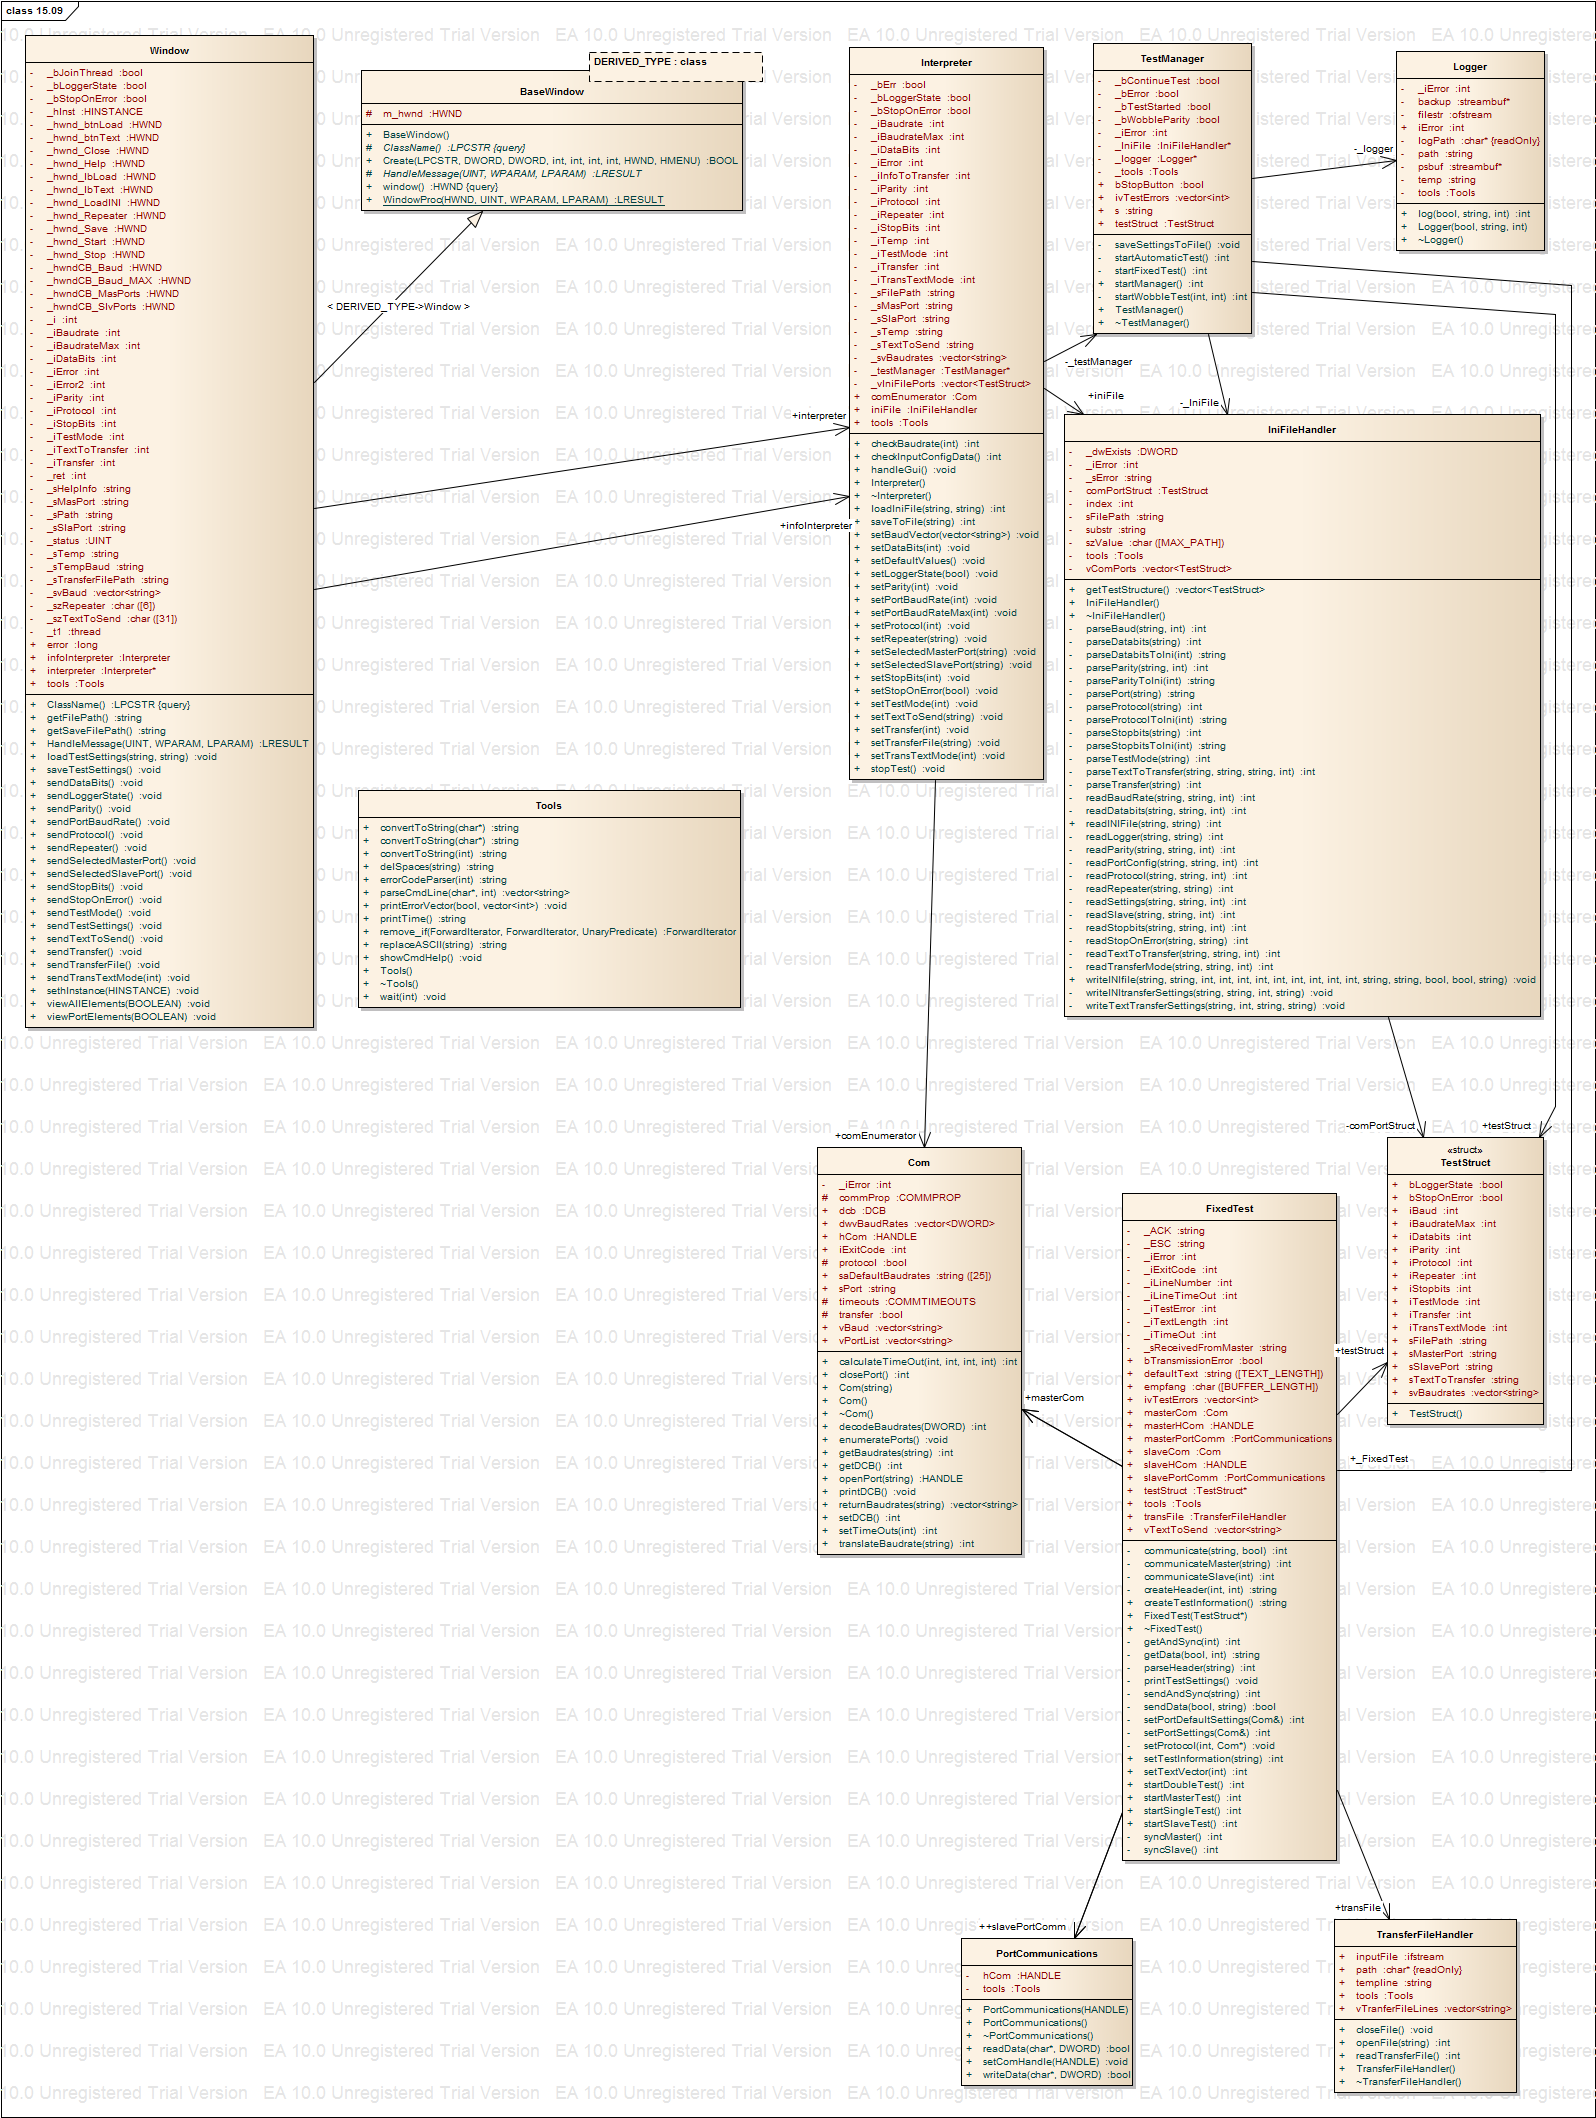
\includegraphics[scale=0.2]{Klassendiagramm_komplett}
  		  \caption{Klassendiagramm}
     \label{KlassenDiagramm}
  \end{center}
\end{figure}



\begin{figure}[h]
  \begin{center}
    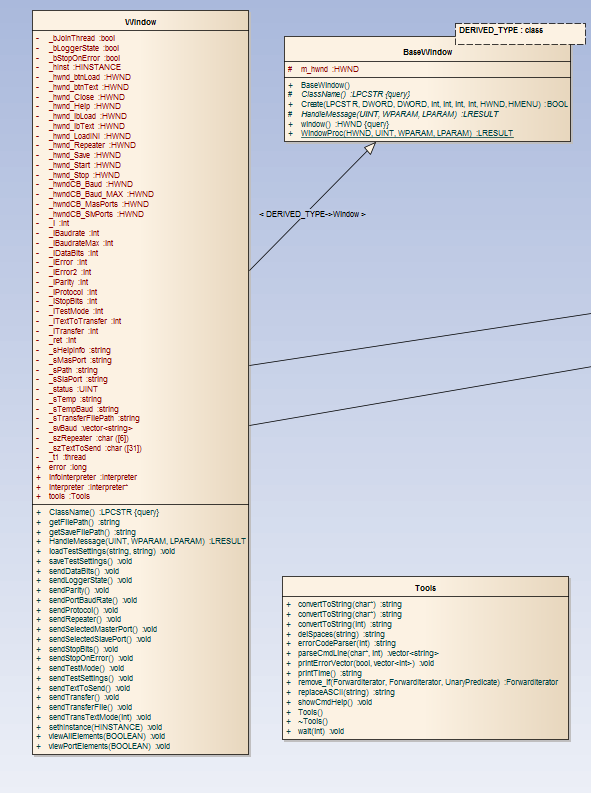
\includegraphics[scale=0.7]{Klassendiagramm1}
  		  \caption{Klassendiagramm Teil 1}
     \label{KlassenDiagramm1}
  \end{center}
\end{figure}

\begin{figure}[h]
  \begin{center}
    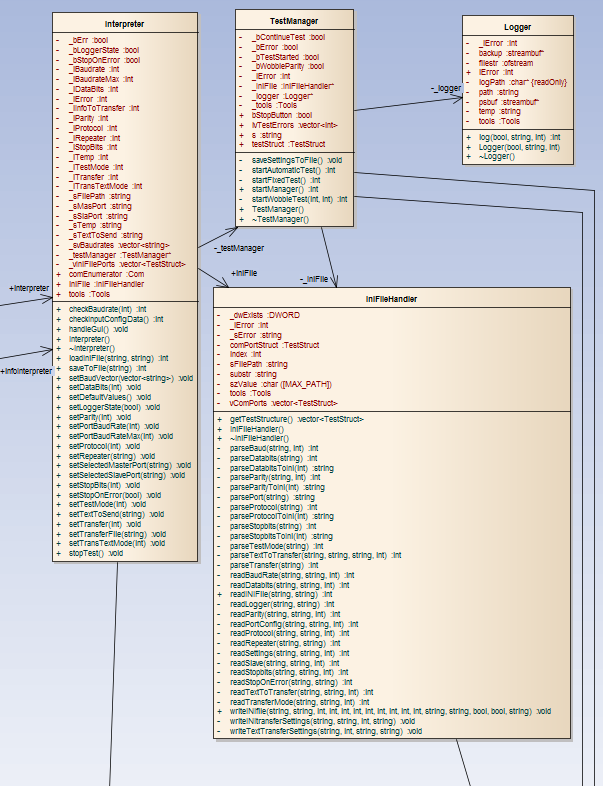
\includegraphics[scale=0.7]{Klassendiagramm2}
  		  \caption{Klassendiagramm Teil 2}
     \label{KlassenDiagramm2}
  \end{center}
\end{figure}

\begin{figure}[h]
  \begin{center}
    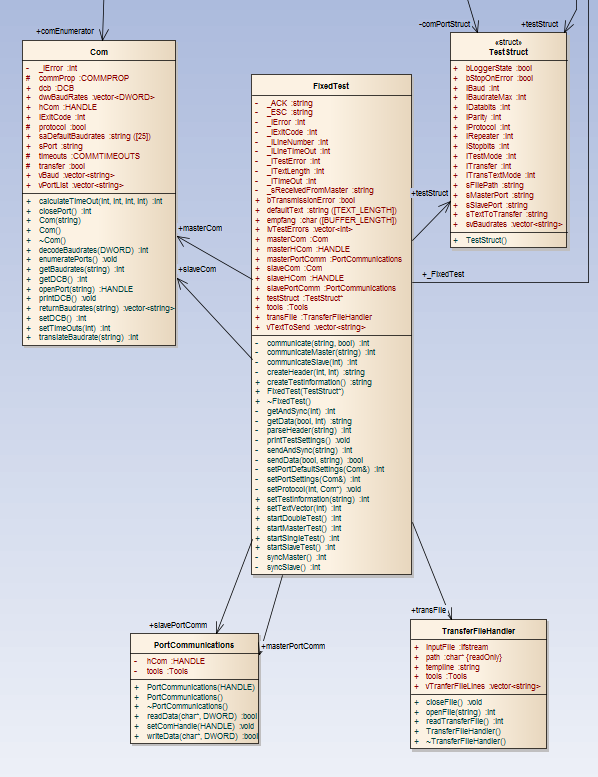
\includegraphics[scale=0.7]{Klassendiagramm3}
  		  \caption{Klassendiagramm Teil 3}
     \label{KlassenDiagramm3}
  \end{center}
\end{figure}